\documentclass[11pt, a4paper]{article}

\usepackage{amsmath}
\usepackage{amsfonts} %Matheschriften
\usepackage{amssymb} %Mathesymbole
%\usepackage{mathptmx} % Einstellung für Schriften und Sonderzeichen in mathematischen Umgebungen
                        % ändert SChriftfont
\usepackage{wasysym} % Stellt diverse Sonderzeichen bereit
\usepackage{siunitx}
\usepackage{float}
% \usepackage{microtype}
\usepackage{graphicx}
\usepackage{hyperref}
\usepackage{xcolor}
\usepackage[section]{placeins}
% allows for temporary adjustment of side margins
\usepackage{changepage}
\usepackage{rotating}


\usepackage[ngerman]{babel}
\addto\captionsngerman{%
 \renewcommand{\abstractname}{Einleitung}}

\title{Versuch 5: Oszilloskop}
\author{Team 2-13: Jascha Fricker, Benedict Brouwer}

\begin{document}
    \maketitle

    \tableofcontents

    \newpage

    \section{Einleitung}
    In diesem Versuch wurden verschiedene RC und LC-Schaltungen mit einem Oszilloskop gemessen.

    \section{Theorie}

    \subsection{Tiefpass}
    Eine Tiefpass besteht aus einem Kondensator mit Kapazität $C$ und einem Widerstand mit Wert $R$. Die Ausgangsspannung wird beim Tiefpass am Kondensator (beim Hochpass am Widerstand) abgegriffen.
    Beim Tiefpass lässt sich aus $R$, $C$ und der Frequenz $f$ die Durchgangskurve, also der Quoteint der Ausgangsspannung $U_{\text{Atp}}$ und der Eingangsspannung $U_{\text{E}}$ 
    \begin{align}
        g_{\text{tp}} &= \frac{U_{\text{Atp}}}{U_{\text{E}}} = \frac{1}{\sqrt{1 + \left( \omega R C \right)}} \\ \label{eq:TiefDurch}
    \end{align}
    berechnen. Auch die Phasenverschiebung
    \begin{align}
        \phi_{\text{tp}} &= \arctan{\frac{1}{\omega R C}} \\ \label{eq:TiefPha}
    \end{align}
    lässt sich theoretisch berechnen.
    Die Grenzfrequenz, bei der die Phasenverschiebung 0 ist, ist somit
    \begin{equation}
        f_{\text{g}} = \frac{1}{2 \pi R C} \,. \label{eq:Grenzfrequenz}
    \end{equation}
    Für das Verhältnis von Eingangsspannung un Ausgangsspannung gilt bei hohen Frequenzen ($f >> f_{\text{g}}$)
    \begin{equation}
        U_{\text{A,TP}}= \frac{1}{RC} \cdot \int U_{\text{E}} \,dt \label{eq:tpint}
    \end{equation}
    Woraus sich die integrierende Wirkung eines Teifpassfilters ableiten lässt

    \subsection{Hochpass}
    Bei niedrigen Frequenzen ($f << f_{\text{g}}$) gilt für das Verhältnis von Eingangsspannung und Ausgangsspannung des Hochpassfilters 
    \begin{equation}
        U_{\text{A,HP}}= RC \cdot \frac{dU_{\text{E}}}{dt} \label{eq:hpdiff}
    \end{equation}
    was die differenzierende Wirkung eine Hochpassfilters erklärt.



    \subsection{Schwingkreis}
    Auch bei einem Serienschwingkreis (Serienschaltuung von Spule und Kondensator) kann die Durchgangskurve
    \begin{equation}
        g_{\text{Ssc}} = \frac{U_{\text{Atp}}}{U_{\text{E}}} = \frac{R}{\sqrt{R^2 + \left( \omega R - \frac{1}{\omega C} \right)^2}} \\
    \end{equation}
    mit dem Ausgangswiderstand $R$, die Phasenverschiebung
    \begin{equation}
        \tan{\phi_{\text{Ssc}}} = \frac{1}{R}\left( \omega L - \frac{1}{\omega C} \right) \\
    \end{equation}
    und die Eigenfreqenz
    \begin{equation}
        f_{\text{Ssc}} = \frac{1}{2 \pi} \sqrt{\frac{1}{L C} - \left(\frac{R}{2L}\right)^2} \,.
    \end{equation}
    berechnen.

    Bei einem Parallelschwinkreis lässt sich die Eigenschwingung
    \begin{equation}
        f_{\text{Psc}} \approx \frac{1}{2 \pi} \sqrt{\frac{1}{R L} - \left(\frac{R^4 C}{2L^3}\right)} \label{eq:koax} \,.
    \end{equation}
    nur ungefähr berechnen.

    Be nicht idealen Schwingkreisen wird die Schwingung gedämpft. Die Schwingung kann durch die Funktion
    \begin{align}
        Q(t) = Q_0 \cdot \cos \left(\omega_E t\right) \cdot \exp \left(-\delta t \right) \label{eq:Q}
        \text{mit Dämpfungskonstante} \delta = \frac{R}{2L} \,
    \end{align}
    beschrieben werden.

    




    \section{Durchführung}
    Zunächst wurde der Tastkopf mit dem dafür vorgesehenen Oszilloskopsignal kallibriert. Da der Tastkopf eine Teilerverhältnis von 10 hat muss also die
    eingestellte Kapazität in etwa 9 mal größer sein als die Kapazität des Kabels und die des Oszilloskops. 
    Anschließend wurde mit einem $6.2(1.2) \si{\nano\farad}$ Kondensator und einem $4.70(47) \si{\kilo\ohm}$ Wiederstand ein Tiefpassfilter aufgebaut. 
    Durch Vergleich von Eingangs und Ausgangsspannung konnte mit diesem Aufbau die Durchlasskurve und Phasenverschiebung gemessen werden.
    Als weiterer Versuch wurde ein Serienschwingkreis mit einem $100.0(1.0) \si{\ohm}$ Wiederstand, einr $2.200(55) \si{\milli\henry}$ Spule und einem $6.2(1.2) \si{\nano\farad}$ Kondensator aufgebaut, mit dem zunächst die Resonanzfrequenz durch einen Frequenzsweep bestimmt wurde.
    Anschliesend wurde abermals die Durchlasskurve und die Dämpfungskonstante bestimmt.
    Zu guter Letzt wurde der Serienschwingkreis in einen Parallelschwingkreis umgebaut mit dem durch Vergleich der Resonanzfrequenzen (abermals mittels eines Frequenzsweeps) die Kapazität eines $10 \si{\metre}$ Koaxkabels bestimmt wurde.

    \section{Ergebnisse und Diskussion}
    \subsection{Tiefpass}
    In Figur \ref{fig:Tiedurchlass} wurde die gemessene Durchlasskurve mit der Theoriekurve \ref{eq:TiefDurch} geplottet. 
    Dabei fällt auf, dass der Fitparameter $RC = 2.95(74) 10^{-5} \si{\ohm\cdot\farad}$ im Konfidenzintervall der angegebenen Größen der Bauteile liegt ($RC_{Bau} = 2.9(0.6)\cdot 10^{-5}$).
    Auch die Messwerte der Phasenverschiebung des Tiefpassfilters \ref{fig:Tiepha}[siehe Figur] lassen sich mit einem im Konfidenzinterval liegenden Fitparamenter ($RC = 3.2(11) \cdot 10^{-5} \si{\ohm\cdot\farad}$) mit der Theoriekurve \ref{eq:TiefPha} fitten.
    Dabei gibt es in den Messdaten zwei Ausreißer mit einer Phasenverschiebung von über $90$° was theoretisch bei einem Tiefpassfilter nicht vorkommen kann.
    Daraus folgt mit Formel \ref{eq:Grenzfrequenz} für die Grenzfrequenzen
    \begin{align}
        f_{grenz,Durch} = 5.4(14) \cdot 10^{3} \\
        f_{grenz,Phase} = 5.0(16) \cdot 10^{3}
    \end{align}

    \begin{figure}[h]
        \centering
        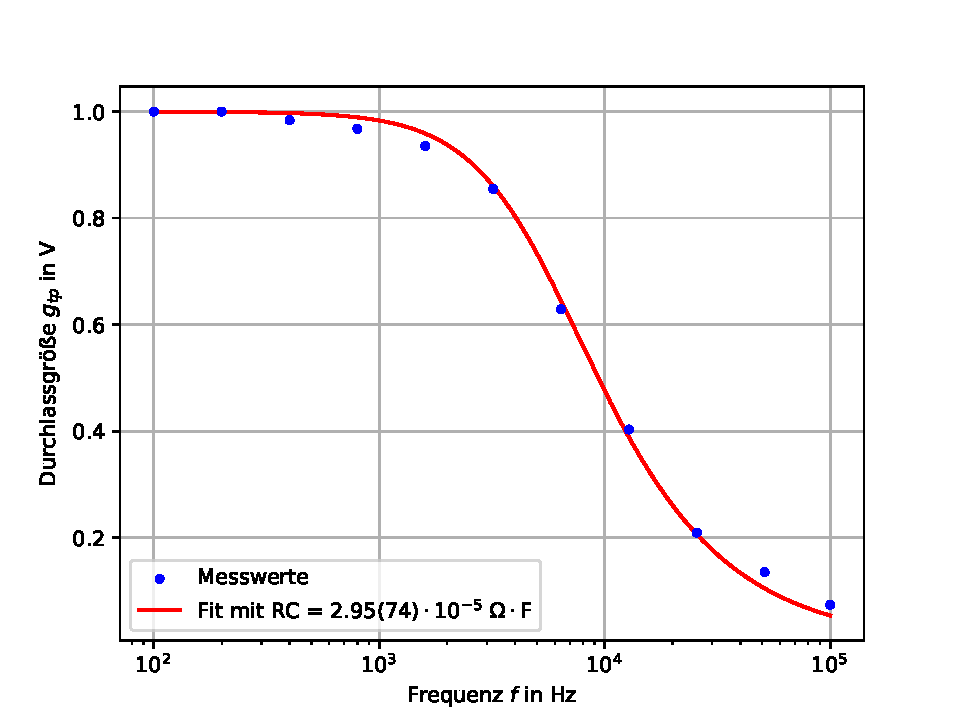
\includegraphics[width=0.8\textwidth]{Tiefdurch.pdf}
        \caption{Durchlasskurve des Tiefpassfilters}
        \label{fig:Tiedurchlass}
    \end{figure}

    \begin{figure}[h]
        \centering
        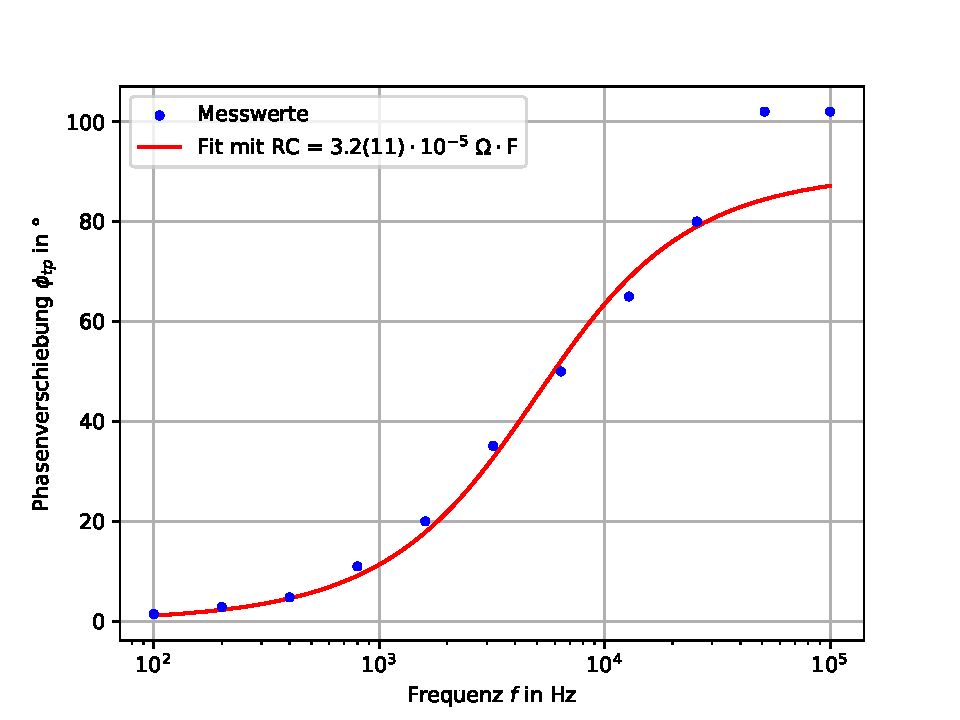
\includegraphics[width=0.8\textwidth]{Tief_Pha.pdf}
        \caption{Phasenverschiebung des Tiefpassfilters bei unterschiedlichen Frequenzen}
        \label{fig:Tiepha}
    \end{figure}
    
    \subsection{Differenzierende und integrierende Wirkung}

    Beim varriieren der Frequenzen bei einem Hoch bzw. Tiefpassfilter fällt nicht nur eine Amplitudenveränderung sondern auch eine Änderug der Signalform an sich auf. Bei Tiefpassfiltern wird das Eingangssignal (blau) bei hohen frequenzen Integriert zum Ausgangssignal (gelb) beeinflusst wie in Bild \ref{im:Tirec} und \ref{im:Titri} zu sehen ist.
    Dies lässt sich mit Formel \ref{eq:tpint} erklären.
    Bei Hochpassfiltern wird das Eingangssignal (blau) zum Ausgangssignal (gelb) bei niedrigen Frequenzen differenziert (mit Formel \ref{eq:hpdiff}) siehe Bild \ref{im:Horec} und \ref{im:Titri}.
    


    \begin{figure}[h]
        \centering
        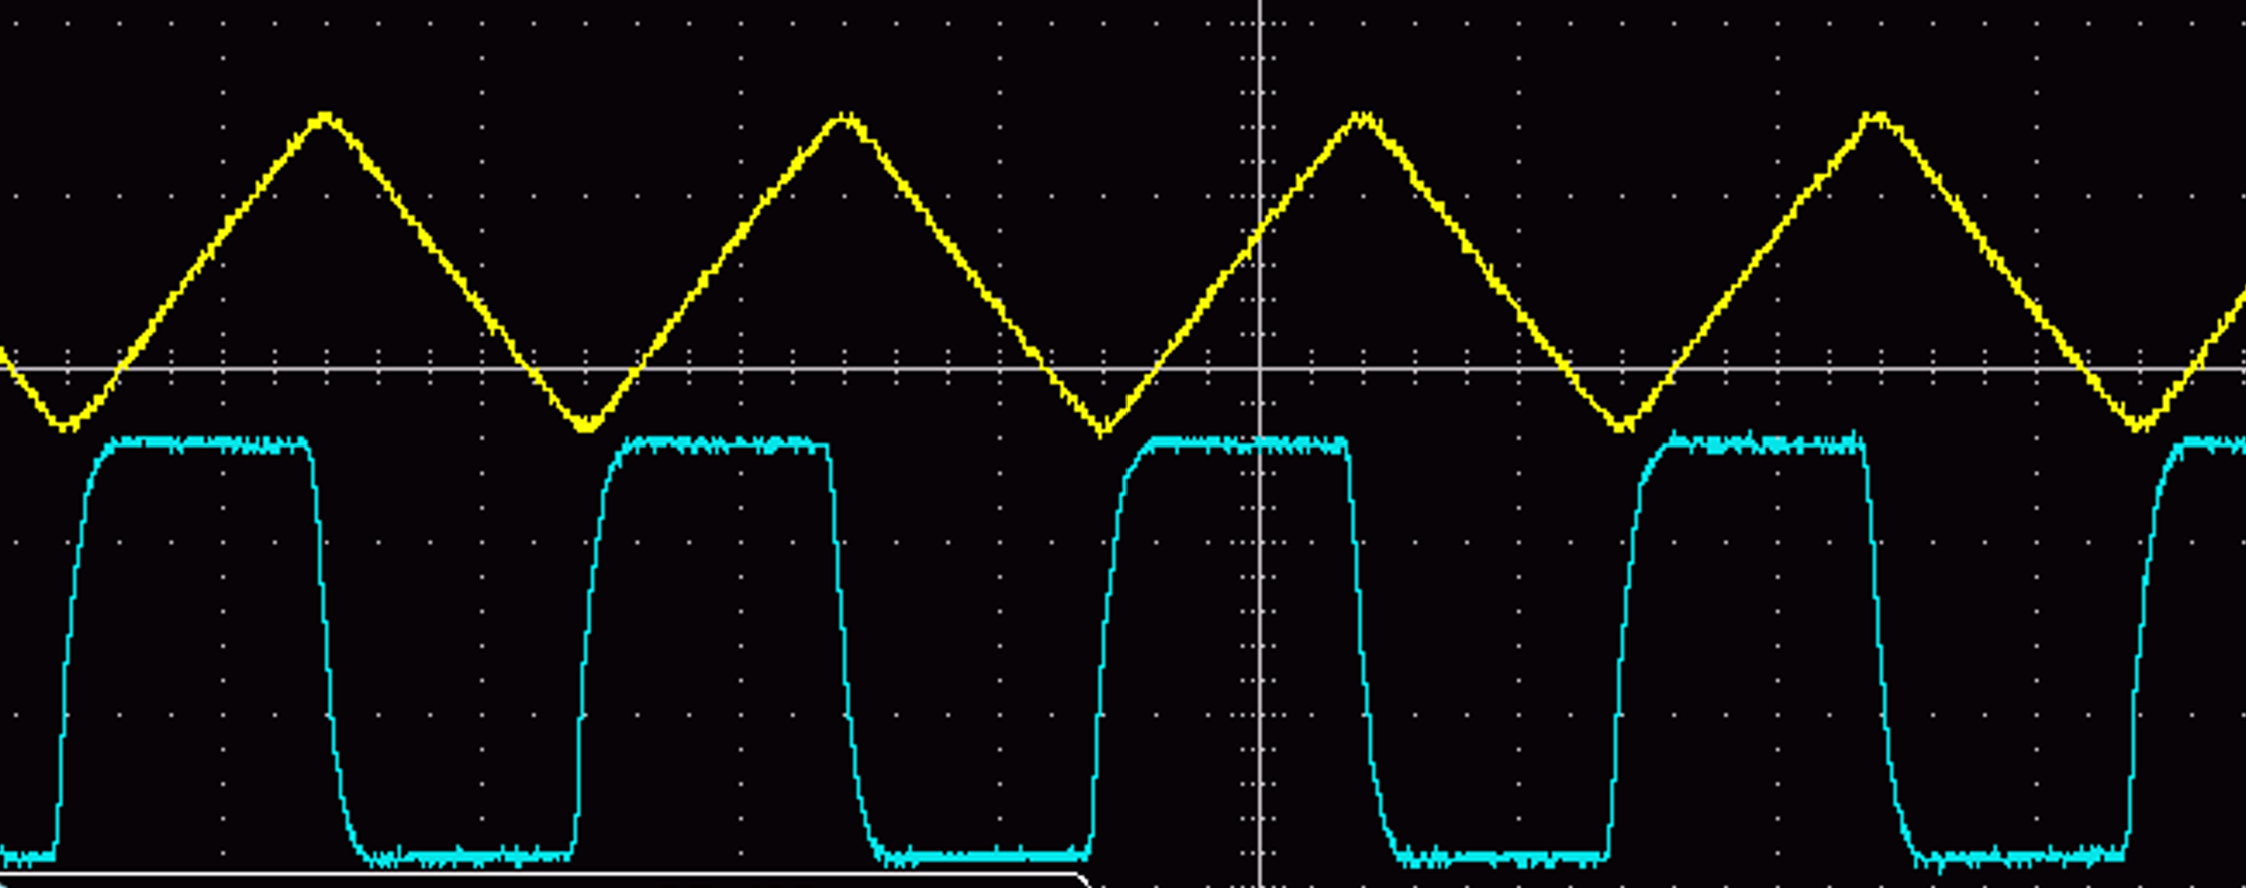
\includegraphics[width=0.8\textwidth]{Tiefpass_Integrierend_rec.png}
        \caption{Tiefpassfilter mit $100 \si{\kilo\hertz}$ Rechtecksignal}
        \label{im:Tirec}
    \end{figure}
    
    \begin{figure}[h]
        \centering
        \includegraphics[width=0.8\textwidth]{Tiefpass_Integrierend_tri.png}
        \caption{Tiefpassfilter mit 100 $\si{\kilo\hertz}$ Dreieckssignal}
        \label{im:Titri}
    \end{figure}
    \begin{figure}[h]
        \centering
        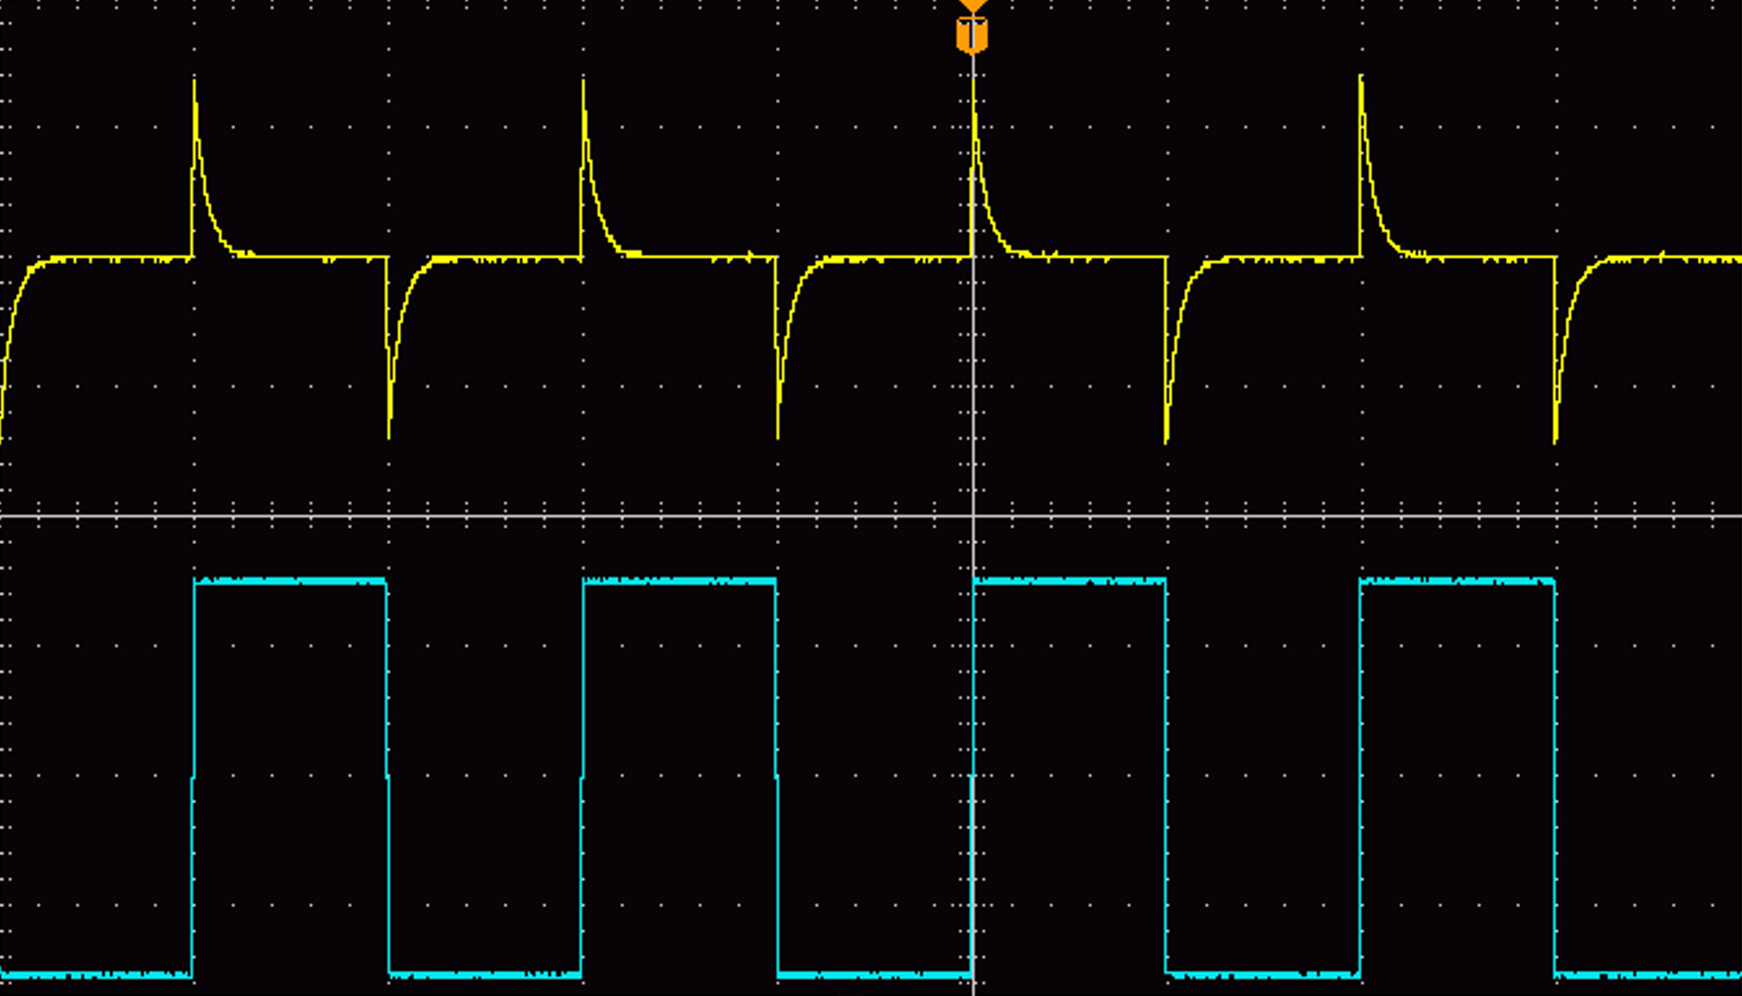
\includegraphics[width=0.8\textwidth]{Hochpass_differenzierend_rec.png}
        \caption{Hochpass mit 1 $\si{\kilo\hertz}$ Rechtecksignal}
        \label{im:Horec}
    \end{figure}
    \begin{figure}[h]
        \centering
        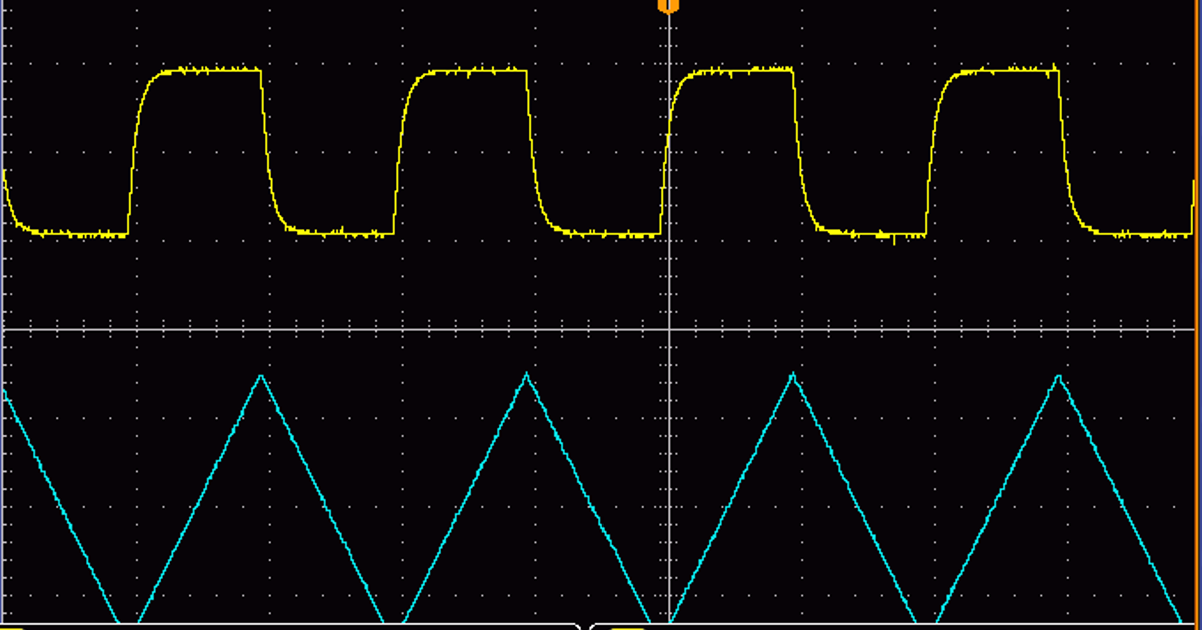
\includegraphics[width=0.8\textwidth]{Hochpass_differenzierend_tri.png}
        \caption{Hochpass mit 1 $\si{\kilo\hertz}$ Dreieckssignal}
        \label{im:Hotri}
    \end{figure}

    \subsection{Serienschwingkreis}
    Mit einem Serienschwingkreis als Filter kann man alle Frequenzen bis auf einen Frequenzbereich herausfiltern. Die Genauigkeit dieses Filters wird durch die Güte $G$ bestimmt. Durch die Messdaten und einen Fit der Theoriekurve wurde, sowohl bei der Durchlasskurve (Siehe Bild: \ref{fig:schwdur}) als auch bei der Phasenverschiebung (Siehe Bild: \ref{fig:schwphas}), die Resonanzfrequenz, die Bandbreite und Güte bestimmt. Diese sind in der Tabelle \ref{tab:./OSZ/schw} aufgeführt.
    
    \input{schw.txt}

    \begin{figure}
        \centering
        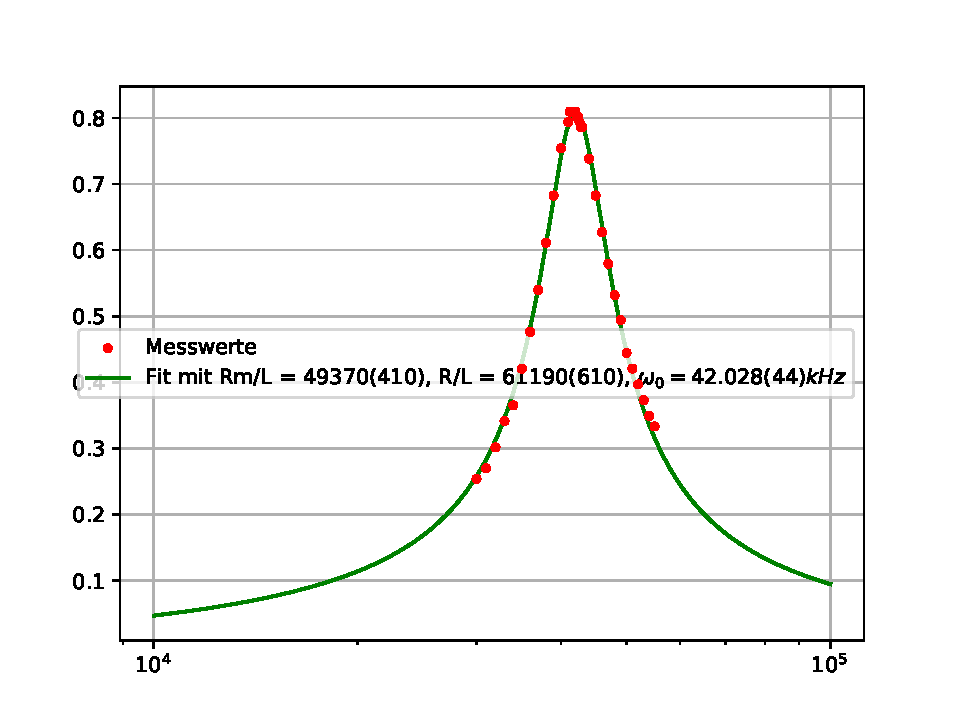
\includegraphics[width=0.8\textwidth]{schwdurch.pdf}
        \caption{Messung Durchlasskurve}
        \label{fig:schwdur}
    \end{figure}

    \begin{figure}
        \centering
        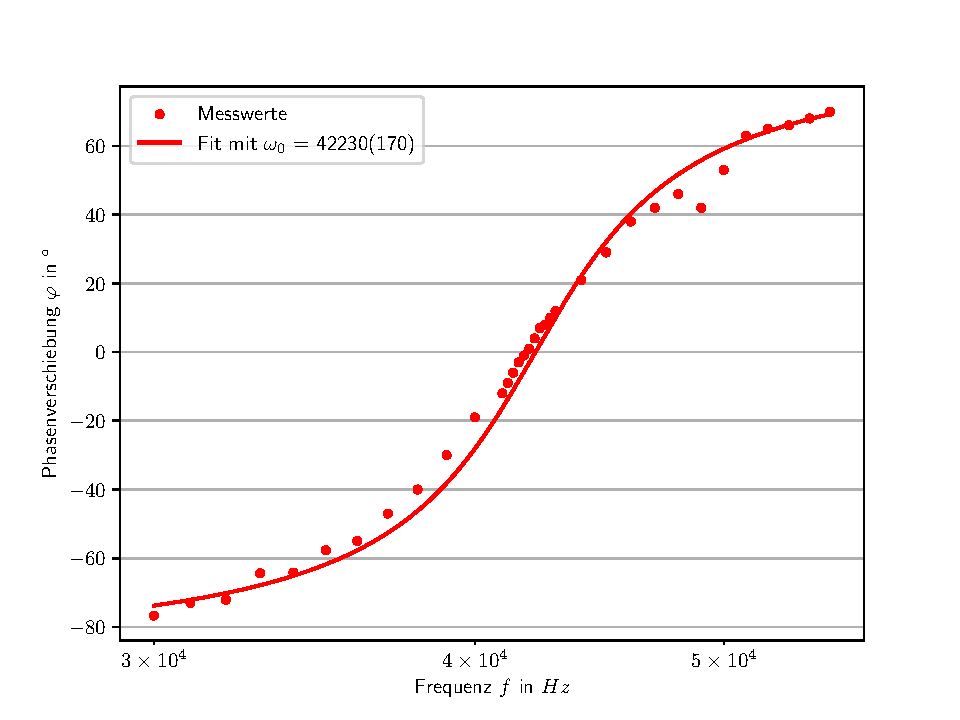
\includegraphics[width=0.8\textwidth]{schwphase.pdf}
        \caption{Messung Phasenverschiebung}
        \label{fig:schwphas}
    \end{figure}

    \paragraph{Bestimmung der Dämpfungskonstante}
    Durch eine Messung der gedämpften Schwingung nach einmaliger Anregung (sehr langsame Rechtecksschwingung), Messwerte und Fit siehe Graph \ref{fig:expfit} konnte die Dämpfungskonstante
    \begin{align}
        \delta = \frac{R}{2L} = 28 630(800) \si{\per\second} \\
        \text{Literaturwert:} 22727 \si{\per\second}
    \end{align}
    bestimmt werden. Zwar liegt der Literaturwert nicht im Konfidenzintervall, aber für die ungenaue Messweise mit nur einer Messreihe ist der Wert sehr nah am Literaturwert.

    \begin{figure}
        \centering
        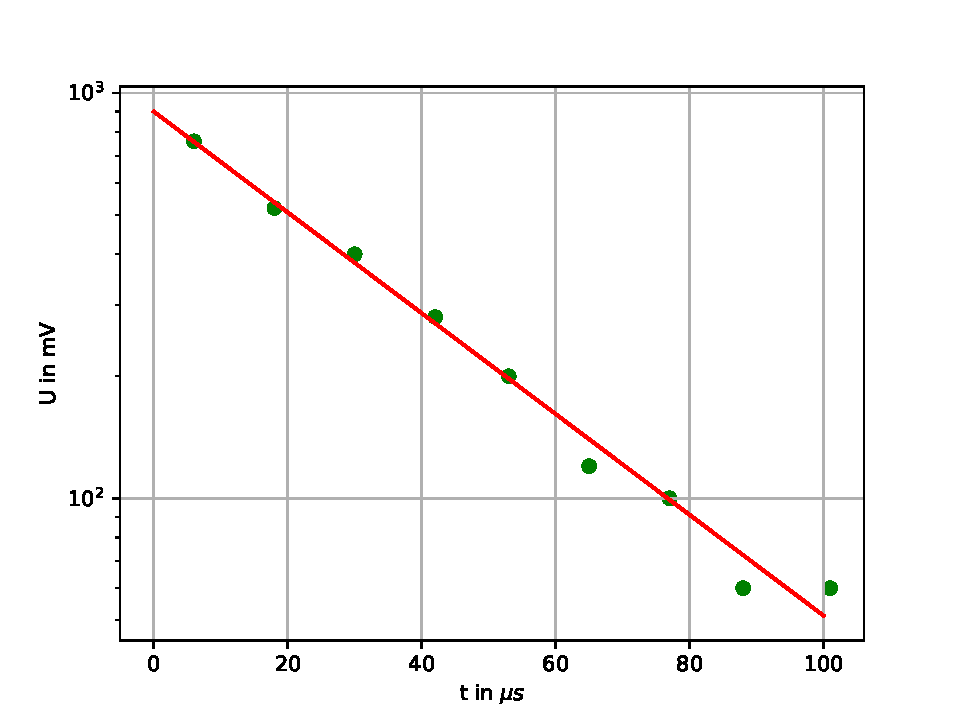
\includegraphics[width=0.8\textwidth]{expfit2.pdf}
        \caption{Messung Dämpfungskonstante}
        \label{fig:expfit}
    \end{figure}

    \subsection{Koaxialkabel}
    Bei deisem Experiment wurden zwei Messwerte gemessen: Die Schwingfrequenz der Parallelschwingkreises ohne Koaxialkabel $f_0 = 42,8 \si{\kilo\hertz}$ und die mit Koaxialkabel $f_K = 42,0 \si{\kilo\hertz}$.
    Mit der Näherung $f_{max} \approx f_0$ kann durch Gleichung \ref{eq:koax} die Kapazität des Koaxialkabels bestimmt werden.
    \begin{align}
        C_0 &= \frac{1}{L \cdot \left(2 pi \cdot f_0 \right)^2} = 6,28  \si{\nano\farad} \\
        C_0 + C_K &= \frac{1}{L \cdot \left(2 pi \cdot f_K \right)^2} = 6,53 \si{\nano\farad} \\
        \Rightarrow C_K &= (6,53 - 6,28) \si{\nano\farad} = 250 \si{\pico\farad}
    \end{align}
    Nach einer Internetrecherche konnte für ein übliches Koaxialkabel ein typischer Wert von ca $100 \si{\pico\farad\per\metre}$ gefunden werden. Damit hätte unser Kabel eine Kapazität von etwa $1 \si{\nano\farad}$. Unser Wert leigt weit daneben, aber die Messweise mit nur zwei werten ist sehr ungenau. Vorallem die Messung der Schwingfrequenz mit dem Osyzilloskp hat große Ungenaugkeit.

    \subsection{Fragen}
    Hochpass, Tiefpass und Schwingkreis sind alles Filter für elektische Signale, die anhand der Frequenz des Signals das Signal mehr oder weniger Dämpfen. Ein Hochpass lässt ab einer bestimmten Grenzfrequenz alle Signale mit größerer Frequenz durch, ein Tiefpass hingegen alle Signale mit kleinerer Frequenz. Mit einem Schwingkreis kann man ein bestimmten Bereich von Frequenzen aussuchen, und andere anderen hinausfiltern. Das Gegenteil vom Schwingkreis wäre ein Notch-Filter, bei dem alle Frequenzen bis auf einen bestimmten Frequenzbereich durchgelassen werden.

    Sowohl ein Feder-Masse-System mit Reibung $\mu$ und Fedekonstante $k$ als auch ein gedämpfter Schwingkreis haben die gleiche lineare Differentialgleichung
    \begin{align}
        \text{Feder:} \quad \frac{d^2x}{dt^2} + \frac{\mu}{m} \frac{dx}{dt} + \frac{k}{m} x = 0 \\
        \text{Schwingkreis:} \quad \frac{d^2Q}{dt^2} + \frac{R}{L} \frac{dQ}{dt} + \frac{1}{LC} Q = 0 \,.
    \end{align}
    So sind auch die Lösungen dieser Gleichungen(eine gedämpften Schwingung) gleich und es können Analogien gebildet werden
    \begin{align}
        \mu = \frac{R}{2L} \quad \text{und} \quad k = \frac{1}{LC} \,.
    \end{align}


    \section{Anhang}
    \subsection{Gaußsche Fehlerfortpflanzung}
    Die Fehlerfortpflanzung wurde mithilfe der Formel
    \begin{align}
        u\left(g \left(x_1, ..., x_n\right)\right) = \sqrt{\sum_{i=1}^n \left( \frac{\partial g }{\partial x_i} \cdot u\left(x_i\right) \right)^2} \label{gauss}
    \end{align}
    berechnet.

    \bibliographystyle{plain}
    \bibliography{literature}

\end{document}